\documentclass[11pt,a4paper]{report}
\usepackage[textwidth=37em,vmargin=30mm]{geometry}
\usepackage{calc,xunicode,amsmath,amssymb,paralist,enumitem,tabu,booktabs,datetime2,xeCJK,xeCJKfntef,listings}
\usepackage{tocloft,fancyhdr,tcolorbox,xcolor,graphicx,eso-pic,xltxtra,xelatexemoji}

\newcommand{\envyear}[0]{2025}
\newcommand{\envdatestr}[0]{2025-08-01}
\newcommand{\envfinaldir}[0]{webdb/2025/20250801/final}

\usepackage[hidelinks]{hyperref}
\hypersetup{
    colorlinks=false,
    pdfpagemode=FullScreen,
    pdftitle={Web Digest - \envdatestr}
}

\setlength{\cftbeforechapskip}{10pt}
\renewcommand{\cftchapfont}{\rmfamily\bfseries\large\raggedright}
\setlength{\cftbeforesecskip}{2pt}
\renewcommand{\cftsecfont}{\sffamily\small\raggedright}

\setdefaultleftmargin{2em}{2em}{1em}{1em}{1em}{1em}

\usepackage{xeCJK,xeCJKfntef}
\xeCJKsetup{PunctStyle=plain,RubberPunctSkip=false,CJKglue=\strut\hskip 0pt plus 0.1em minus 0.05em,CJKecglue=\strut\hskip 0.22em plus 0.2em}
\XeTeXlinebreaklocale "zh"
\XeTeXlinebreakskip = 0pt


\setmainfont{Brygada 1918}
\setromanfont{Brygada 1918}
\setsansfont{IBM Plex Sans}
\setmonofont{JetBrains Mono NL}
\setCJKmainfont{Noto Serif CJK SC}
\setCJKromanfont{Noto Serif CJK SC}
\setCJKsansfont{Noto Sans CJK SC}
\setCJKmonofont{Noto Sans CJK SC}

\setlength{\parindent}{0pt}
\setlength{\parskip}{8pt}
\linespread{1.15}

\lstset{
	basicstyle=\ttfamily\footnotesize,
	numbersep=5pt,
	backgroundcolor=\color{black!5},
	showspaces=false,
	showstringspaces=false,
	showtabs=false,
	tabsize=2,
	captionpos=b,
	breaklines=true,
	breakatwhitespace=true,
	breakautoindent=true,
	linewidth=\textwidth
}






\newcommand{\coverpic}[2]{
    % argv: itemurl, authorname
    Cover photo by #2~~(\href{#1}{#1})
}
\newcommand{\makeheader}[0]{
    \begin{titlepage}
        % \newgeometry{hmargin=15mm,tmargin=21mm,bmargin=12mm}
        \begin{center}
            
            \rmfamily\scshape
            \fontspec{BaskervilleF}
            \fontspec{Old Standard}
            \fontsize{59pt}{70pt}\selectfont
            WEB\hfill DIGEST
            
            \vfill
            % \vskip 30pt
            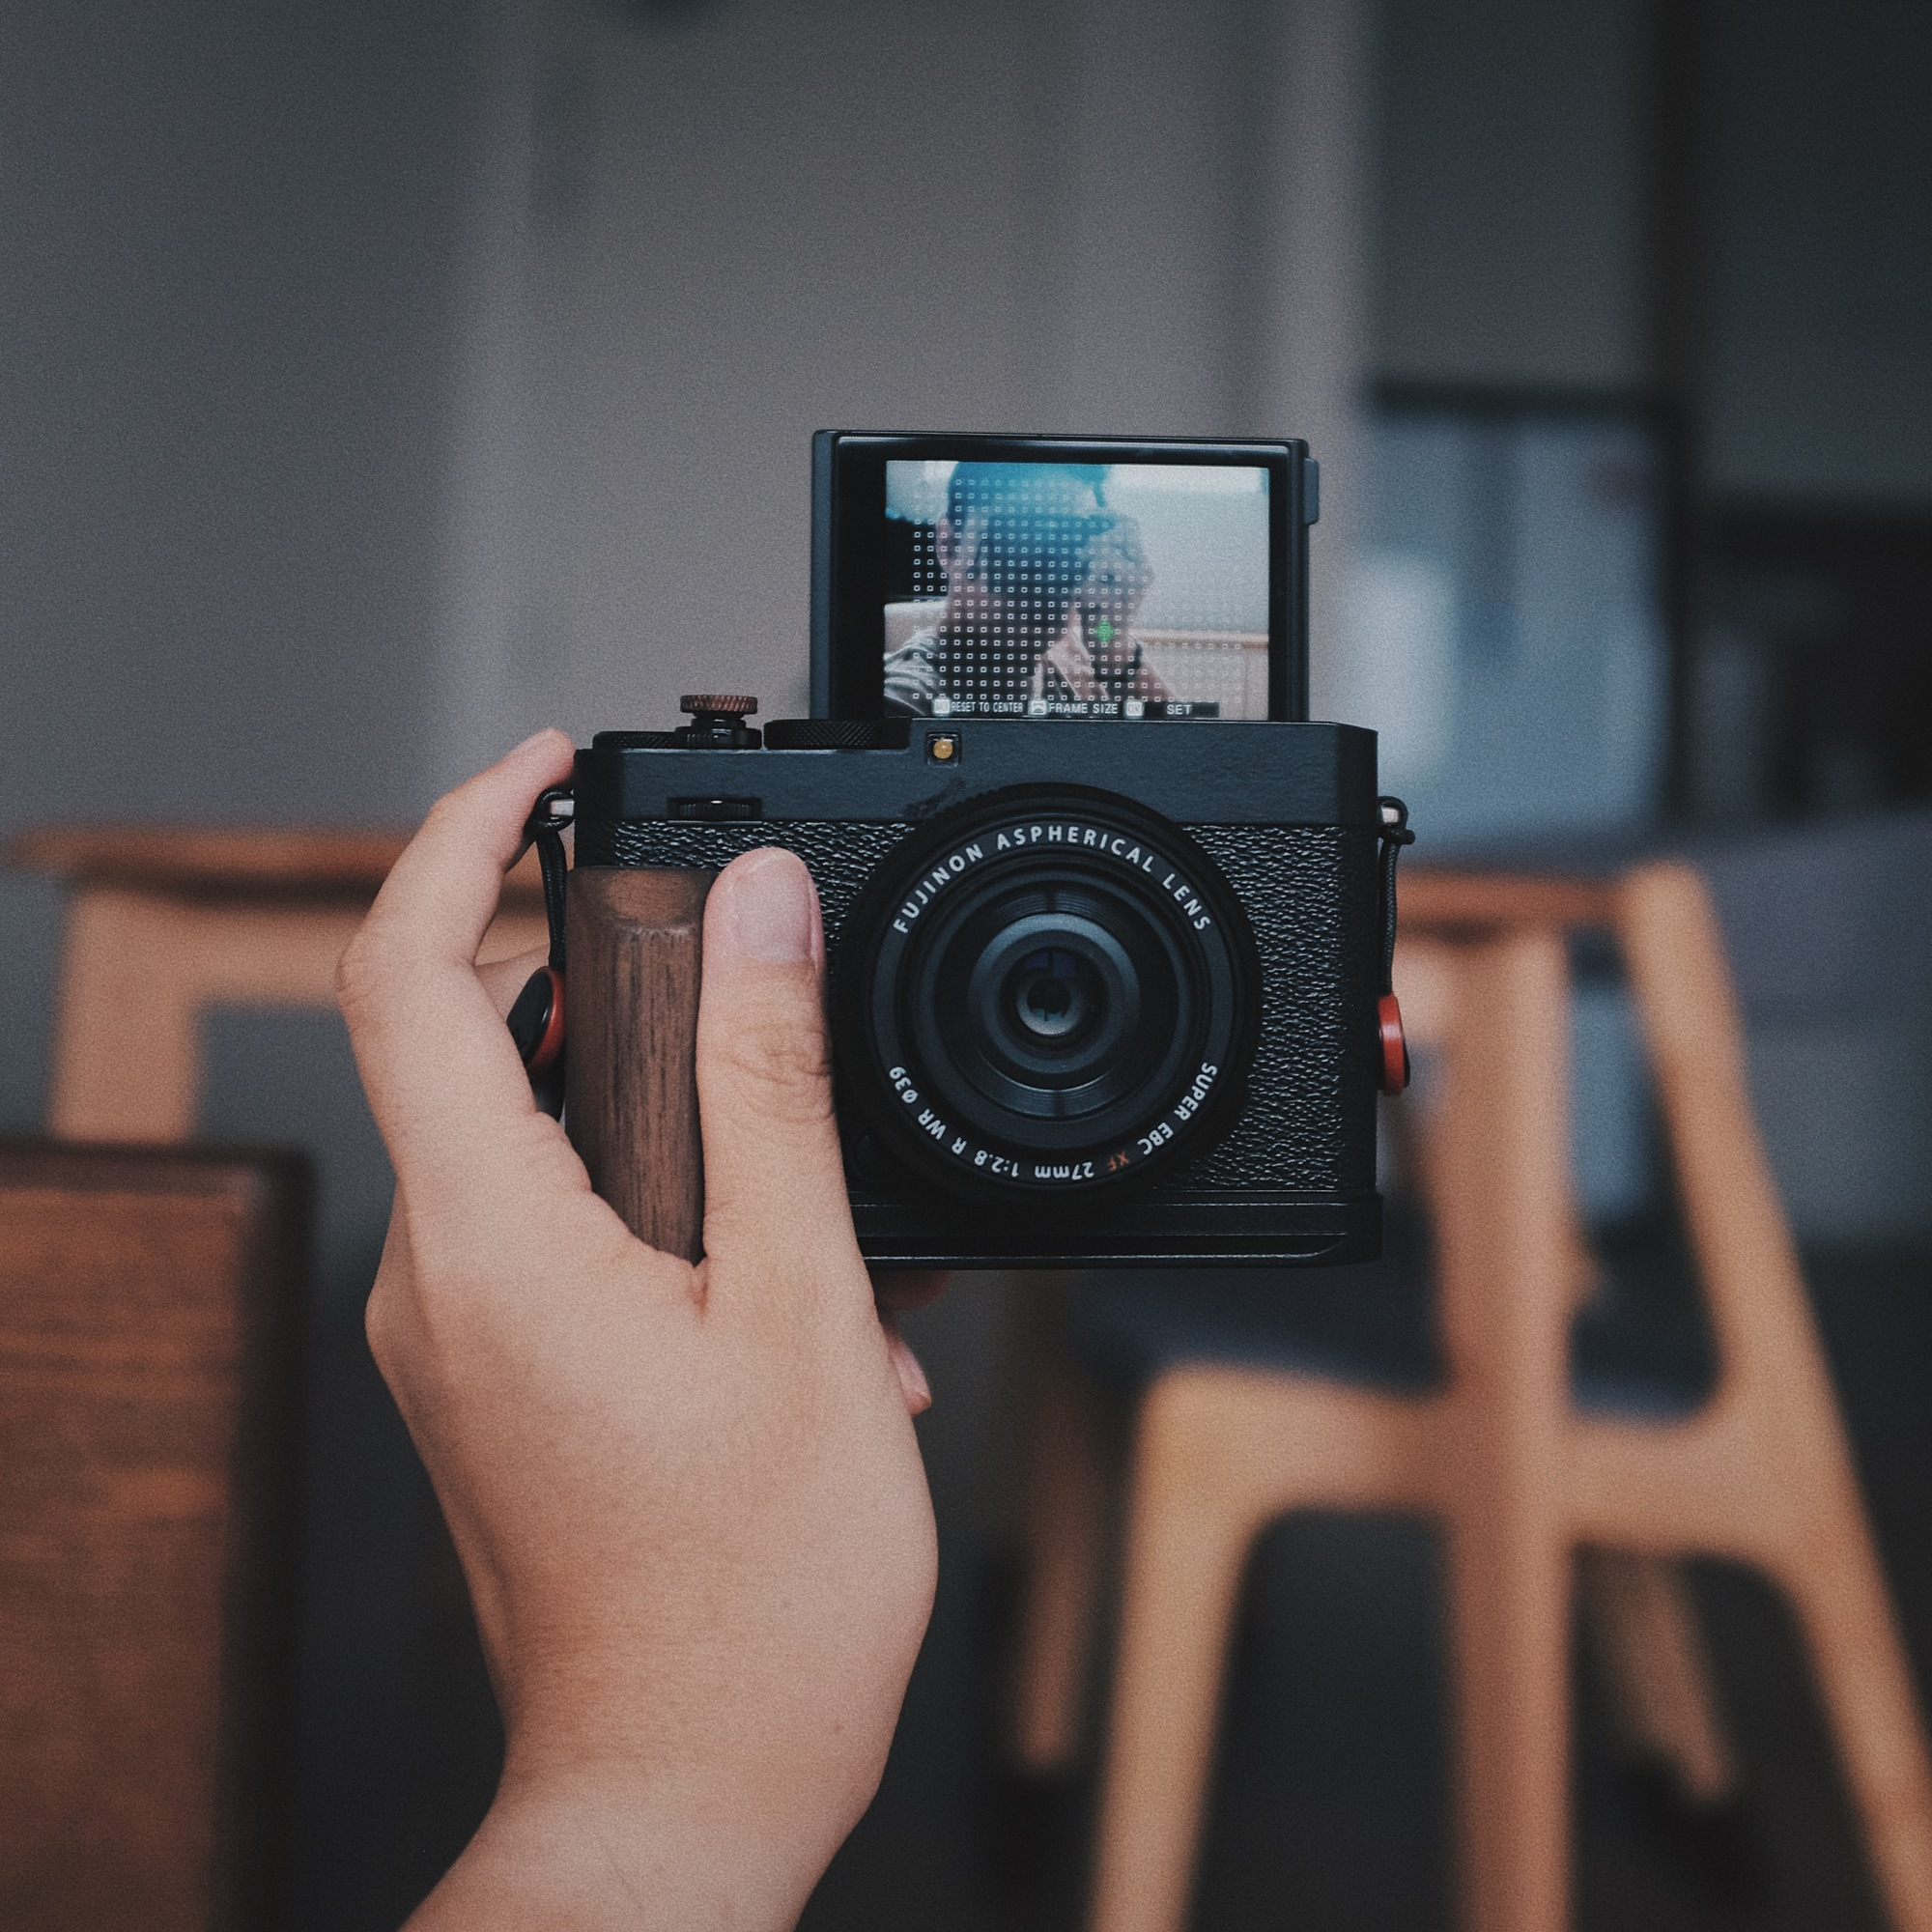
\includegraphics[width=\linewidth]{\envfinaldir/coverpic-prod.jpg}\par
            % \vskip 30pt
            \vfill

            \normalsize\rmfamily\scshape
            \copyright{} The Web Digest Project \hfill\large \envdatestr
        \end{center}
    \end{titlepage}
    % \restoregeometry
}
\newcommand{\simplehref}[1]{%
    \textcolor{blue!80!green}{\href{#1}{#1}}%
}
\renewcommand{\contentsname}{\center\Huge\sffamily\bfseries Contents\par\vskip 20pt}
\newcounter{ipartcounter}
\setcounter{ipartcounter}{0}
\newcommand{\ipart}[1]{
    % \vskip 20pt
    \clearpage
    \stepcounter{ipartcounter}
    \phantomsection
    \addcontentsline{toc}{chapter}{#1}
    % \begin{center}
    %     \Huge
    %     \sffamily\bfseries
    %     #1
    % \end{center}
    % \vskip 20pt plus 7pt
}
\newcounter{ichaptercounter}
\setcounter{ichaptercounter}{0}
\newcommand{\ichapter}[1]{
    % \vskip 20pt
    \clearpage
    \stepcounter{ichaptercounter}
    \phantomsection
    \addcontentsline{toc}{section}{\numberline{\arabic{ichaptercounter}}#1}
    \begin{center}
        \Huge
        \sffamily\bfseries
        #1
    \end{center}
    \vskip 20pt plus 7pt
}
\newcommand{\entrytitlefont}[1]{\subsection*{\raggedright\Large\sffamily\bfseries#1}}
\newcommand{\entryitemGeneric}[2]{
    % argv: title, url
    \parbox{\linewidth}{
        \entrytitlefont{#1}\par\vskip 5pt
        \footnotesize\ttfamily\mdseries
        \simplehref{#2}
    }\vskip 11pt plus 11pt minus 1pt
}
\newcommand{\entryitemGithub}[3]{
    % argv: title, url, desc
    \parbox{\linewidth}{
        \entrytitlefont{#1}\par\vskip 5pt
        \footnotesize\ttfamily\mdseries
        \simplehref{#2}\par\vskip 5pt
        \small\rmfamily\mdseries#3
    }\vskip 11pt plus 11pt minus 1pt
}
\newcommand{\entryitemAp}[3]{
    % argv: title, url, desc
    \parbox{\linewidth}{
        \entrytitlefont{#1}\par\vskip 5pt
        \footnotesize\ttfamily\mdseries
        \simplehref{#2}\par\vskip 5pt
        \small\rmfamily\mdseries#3
    }\vskip 11pt plus 11pt minus 1pt
}
\newcommand{\entryitemHackernews}[3]{
    % argv: title, hnurl, rawurl
    % \parbox{\linewidth}{
    %     \entrytitlefont{#1}\par\vskip 5pt
    %     \footnotesize\ttfamily\mdseries
    %     \simplehref{#3}\par
    %     \textcolor{black!50}{\href{#2}{#2}}
    % }\vskip 11pt plus 11pt minus 1pt
    \begin{minipage}{\linewidth}
            \entrytitlefont{#1}\par\vskip 5pt
            \footnotesize\ttfamily\mdseries
            \simplehref{#3}\par
            \textcolor{black!50}{\href{#2}{#2}}
    \end{minipage}\par\vskip 11pt plus 11pt minus 1pt
}







\begin{document}

\makeheader

\tableofcontents\clearpage




\ipart{Developers}
\ichapter{Hacker News}
\entryitemTwoLinks{Denver rent is back to 2022 prices after 20k new units hit the market}{https://news.ycombinator.com/item?id=44749772}{https://denverite.com/2025/07/25/denver-rent-prices-drop-q2/}

\entryitemTwoLinks{Slow}{https://news.ycombinator.com/item?id=44748934}{https://michaelnotebook.com/slow/index.html}

\entryitemTwoLinks{AI is a floor raiser, not a ceiling raiser}{https://news.ycombinator.com/item?id=44747634}{https://elroy.bot/blog/2025/07/29/ai-is-a-floor-raiser-not-a-ceiling-raiser.html}

\entryitemTwoLinks{Gemini Embedding: Powering RAG and context engineering}{https://news.ycombinator.com/item?id=44747457}{https://developers.googleblog.com/en/gemini-embedding-powering-rag-context-engineering/}

\entryitemTwoLinks{QUIC for the kernel}{https://news.ycombinator.com/item?id=44746948}{https://lwn.net/Articles/1029851/}

\entryitemTwoLinks{Ubiquiti launches UniFi OS Server for self-hosting}{https://news.ycombinator.com/item?id=44746603}{https://lazyadmin.nl/home-network/unifi-os-server/}

\entryitemTwoLinks{U.S. senators introduce new pirate site blocking bill, "Block BEARD"}{https://news.ycombinator.com/item?id=44746334}{https://torrentfreak.com/u-s-senators-introduce-new-pirate-site-blocking-bill-block-beard/}

\entryitemTwoLinks{MacBook Pro Insomnia}{https://news.ycombinator.com/item?id=44745897}{https://manuel.bernhardt.io/posts/2025-07-24-macbook-pro-insomnia}

\entryitemTwoLinks{Releasing open weights for FLUX.1 Krea}{https://news.ycombinator.com/item?id=44745555}{https://www.krea.ai/blog/flux-krea-open-source-release}

\entryitemTwoLinks{So you're a manager now}{https://news.ycombinator.com/item?id=44745123}{https://scottkosman.com/post/blog/so-youre-a-manager-now/}

\entryitemTwoLinks{Many countries that said no to ChatControl in 2024 are now undecided}{https://news.ycombinator.com/item?id=44744715}{https://digitalcourage.social/@echo\_pbreyer/114946559233051667}

\entryitemTwoLinks{Introduction to Computer Music}{https://news.ycombinator.com/item?id=44744578}{https://cmtext.com/}

\entryitemTwoLinks{How was the Universal Pictures 1936 opening logo created?}{https://news.ycombinator.com/item?id=44744454}{https://movies.stackexchange.com/questions/128020/how-was-the-universal-pictures-1936-opening-logo-created}

\entryitemTwoLinks{I tried Servo}{https://news.ycombinator.com/item?id=44744324}{https://www.spacebar.news/servo-undercover-web-browser-engine/}

\entryitemTwoLinks{Hawley and Democrats vote to advance congressional stock trading ban}{https://news.ycombinator.com/item?id=44744096}{https://www.cbsnews.com/news/hawley-democrats-vote-stock-trading-ban-committee/}

\entryitemTwoLinks{I know when you're vibe coding}{https://news.ycombinator.com/item?id=44742251}{https://alexkondov.com/i-know-when-youre-vibe-coding/}

\entryitemTwoLinks{Classic Common Desktop Environment coming to OpenBSD}{https://news.ycombinator.com/item?id=44741539}{https://undeadly.org/cgi?action=article;sid=20250730080301}

\entryitemTwoLinks{Microsoft became incompetent in IT}{https://news.ycombinator.com/item?id=44741442}{https://mikekaganski.wordpress.com/2025/07/25/microsoft-anybody-home/}

\entryitemTwoLinks{Figma will IPO on July 31}{https://news.ycombinator.com/item?id=44740222}{https://www.figma.com/blog/ipo-pricing/}

\entryitemTwoLinks{Ollama's new app}{https://news.ycombinator.com/item?id=44739632}{https://ollama.com/blog/new-app}


\ipart{Developers~~~~(zh-Hans)}
\ichapter{Solidot}
\entryitemGeneric{\hskip 0pt{}高铁的环境影响}{https://www.solidot.org/story?sid=81939}

\entryitemGeneric{\hskip 0pt{}人类每天在室内环境吸入逾 7 万个微塑料}{https://www.solidot.org/story?sid=81938}

\entryitemGeneric{\hskip 0pt{}人工甜味剂显著增加罹患糖尿病风险}{https://www.solidot.org/story?sid=81937}

\entryitemGeneric{\hskip 0pt{}研究显示限制 Google 付费成为默认搜索引擎能降低其市场份额}{https://www.solidot.org/story?sid=81936}

\entryitemGeneric{\hskip 0pt{}网信办约谈英伟达}{https://www.solidot.org/story?sid=81935}

\entryitemGeneric{\hskip 0pt{}AI 生成的代码近半包含安全漏洞}{https://www.solidot.org/story?sid=81934}

\entryitemGeneric{\hskip 0pt{}Vivo 宣布了用 Rust 开发的 BlueOS}{https://www.solidot.org/story?sid=81933}

\entryitemGeneric{\hskip 0pt{}澳大利亚儿童社媒禁令扩大到 YouTube}{https://www.solidot.org/story?sid=81932}

\entryitemGeneric{\hskip 0pt{}地球各大洲都经历淡水流失}{https://www.solidot.org/story?sid=81931}

\entryitemGeneric{\hskip 0pt{}愤怒的玩家对 Visa 和 Mastercard 的客服发动 DDoS 攻击}{https://www.solidot.org/story?sid=81930}

\entryitemGeneric{\hskip 0pt{}猫会让 AI 困惑}{https://www.solidot.org/story?sid=81929}

\entryitemGeneric{\hskip 0pt{}Google 鼓励员工使用 AI}{https://www.solidot.org/story?sid=81928}

\entryitemGeneric{\hskip 0pt{}Futurehome 申请破产后推送固件移除设备本地功能强推订阅制}{https://www.solidot.org/story?sid=81927}

\entryitemGeneric{\hskip 0pt{}微软承认它无法保障欧洲国家的数字主权}{https://www.solidot.org/story?sid=81926}

\entryitemGeneric{\hskip 0pt{}调查发现六成美国人将 AI 用于搜索 37\% 的人用于工作}{https://www.solidot.org/story?sid=81925}

\entryitemGeneric{\hskip 0pt{}印度对美智能手机出货量首次超过中国}{https://www.solidot.org/story?sid=81924}

\entryitemGeneric{\hskip 0pt{}Opera 指控微软使用反竞争策略推广自家浏览器 Edge }{https://www.solidot.org/story?sid=81923}

\entryitemGeneric{\hskip 0pt{}微软封禁 LibreOffice 开发者账号}{https://www.solidot.org/story?sid=81922}

\entryitemGeneric{\hskip 0pt{}俄罗斯堪察加半岛发生 M8.8 级地震}{https://www.solidot.org/story?sid=81921}

\entryitemGeneric{\hskip 0pt{}成人网站指控 Meta 下载和做种成人视频}{https://www.solidot.org/story?sid=81920}\ichapter{V2EX}
\entryitemGeneric{\hskip 0pt{}[职场话题] 基本工资 5k+绩效 20k=25k 的合同有没有坑?}{https://www.v2ex.com/t/1149150}

\entryitemGeneric{\hskip 0pt{}[服务器] ububtu 终于退坑了。}{https://www.v2ex.com/t/1149149}

\entryitemGeneric{\hskip 0pt{}[Solana] 哪个大哥在拉盘啊.}{https://www.v2ex.com/t/1149148}

\entryitemGeneric{\hskip 0pt{}[分享创造] 使用 go 和仓颉重构了整个 PHP}{https://www.v2ex.com/t/1149147}

\entryitemGeneric{\hskip 0pt{}[随想] 去一座新的城市,开始一段新的旅途}{https://www.v2ex.com/t/1149146}

\entryitemGeneric{\hskip 0pt{}[问与答] 很好奇,兼职收入你们会申报个税吗?高达 20\%甚至 40\%的税.....}{https://www.v2ex.com/t/1149145}

\entryitemGeneric{\hskip 0pt{}[宽带症候群] 都 2025 年了,你根本不需要 mesh 组网}{https://www.v2ex.com/t/1149144}

\entryitemGeneric{\hskip 0pt{}[Apple] 想买个老苹果玩越狱 最佳选择是}{https://www.v2ex.com/t/1149143}

\entryitemGeneric{\hskip 0pt{}[分享创造] 一种基于 EasyVtuber 和 Stable Diffusion 的零成本虚拟形象直播方案}{https://www.v2ex.com/t/1149142}

\entryitemGeneric{\hskip 0pt{}[酷工作] 微软苏州实习机会}{https://www.v2ex.com/t/1149141}

\entryitemGeneric{\hskip 0pt{}[分享创造] MPL: MMD Pose Language 用编程的方式做纸片人动画}{https://www.v2ex.com/t/1149140}

\entryitemGeneric{\hskip 0pt{}[Solana] v2ex 在手机浏览器上绑定 sol 地址不够丝滑}{https://www.v2ex.com/t/1149139}

\entryitemGeneric{\hskip 0pt{}[分享发现] Qwen3-Coder-30B-A3B-Instruct 来了}{https://www.v2ex.com/t/1149137}

\entryitemGeneric{\hskip 0pt{}[Vue.js] VUE 开发求助}{https://www.v2ex.com/t/1149136}

\entryitemGeneric{\hskip 0pt{}[程序员] 广州汇丰软件的年假可以换成钱吗?}{https://www.v2ex.com/t/1149135}

\entryitemGeneric{\hskip 0pt{}[分享创造] Pivo - 以任务为中心的 Vibe 编程环境}{https://www.v2ex.com/t/1149134}

\entryitemGeneric{\hskip 0pt{}[生活] 分享一道简单好吃的菜 红葱头蒸鸡腿肉}{https://www.v2ex.com/t/1149133}

\entryitemGeneric{\hskip 0pt{}[程序员] 应该选择什么样的技术栈呢? React or Vue?}{https://www.v2ex.com/t/1149132}

\entryitemGeneric{\hskip 0pt{}[NAS] Plex 对 DLNA 的限制是更严格吗?}{https://www.v2ex.com/t/1149131}

\entryitemGeneric{\hskip 0pt{}[问与答] 这样的公司还能呆吗?}{https://www.v2ex.com/t/1149130}

\entryitemGeneric{\hskip 0pt{}[程序员] box2d 3.1.0 + SFML 3.0.0 游戏项目开发}{https://www.v2ex.com/t/1149129}

\entryitemGeneric{\hskip 0pt{}[分享发现] 年底打算去日本旅行并办目的地婚礼, V 友们有什么推荐和经验分享吗}{https://www.v2ex.com/t/1149128}

\entryitemGeneric{\hskip 0pt{}[问与答] 动态血糖仪有推荐的吗?}{https://www.v2ex.com/t/1149127}

\entryitemGeneric{\hskip 0pt{}[分享创造] 纯 flutter app 开发, web 菜鸟级选手,做了 1 个入门级网站}{https://www.v2ex.com/t/1149126}

\entryitemGeneric{\hskip 0pt{}[推广] 发现一个用起来很丝滑的 emby 硬盘商业服}{https://www.v2ex.com/t/1149125}

\entryitemGeneric{\hskip 0pt{}[生活] 每个月收入 5-7 万 你会选择买房子还是租房子?}{https://www.v2ex.com/t/1149124}

\entryitemGeneric{\hskip 0pt{}[问与答] 微信电脑版这是又搞什么幺蛾子,原本的 WeChat Files 不用,又新建一个 xwechat\_files}{https://www.v2ex.com/t/1149123}

\entryitemGeneric{\hskip 0pt{}[宽带症候群] 现在有卖内置魔法账号的路由器吗?}{https://www.v2ex.com/t/1149122}

\entryitemGeneric{\hskip 0pt{}[宽带症候群] 北京移动宽带路由器拨号,得不到 ipv6 地址了}{https://www.v2ex.com/t/1149120}

\entryitemGeneric{\hskip 0pt{}[生活] 最近看到关于 2023 年武汉大学肖同学被告性骚扰的事有感。}{https://www.v2ex.com/t/1149118}

\entryitemGeneric{\hskip 0pt{}[Solana] \$V2EX 进场, 详解 OKX 交易所注册+OKX 钱包购买\$V2EX}{https://www.v2ex.com/t/1149117}

\entryitemGeneric{\hskip 0pt{}[分享发现] 我不相信天下有讲不明白的道理!}{https://www.v2ex.com/t/1149116}

\entryitemGeneric{\hskip 0pt{}[Solana] 折腾了好久,终于绑定好钱包地址了,可以尝试打赏与被打赏了。}{https://www.v2ex.com/t/1149114}

\entryitemGeneric{\hskip 0pt{}[推广] 基于 SpringAi 的模块化设计 Agent 框架,像搭积木一样搭建 Agent。}{https://www.v2ex.com/t/1149113}

\entryitemGeneric{\hskip 0pt{}[Apple] 想把 NAS 卖了换 Mac mini M1 当服务器...}{https://www.v2ex.com/t/1149112}

\entryitemGeneric{\hskip 0pt{}[旅行] 游记分享 港澳深大湾区风球中旅程}{https://www.v2ex.com/t/1149111}

\entryitemGeneric{\hskip 0pt{}[问与答] Claude Code 目前还没有很方便的 Rollback/Checkpoint 吗?}{https://www.v2ex.com/t/1149110}

\entryitemGeneric{\hskip 0pt{}[分享发现] 这个是被漏洞上传了吗?}{https://www.v2ex.com/t/1149109}

\entryitemGeneric{\hskip 0pt{}[Solana] v 站上打赏好像不需要网络费用,这是有合作么}{https://www.v2ex.com/t/1149107}

\entryitemGeneric{\hskip 0pt{}[问与答] 请问有哪些手段可以判断访问流量是真人还是 bot ?}{https://www.v2ex.com/t/1149106}

\entryitemGeneric{\hskip 0pt{}[iOS] [有偿] Ios 集成 zerotier-demo}{https://www.v2ex.com/t/1149104}

\entryitemGeneric{\hskip 0pt{}[全球工单系统] 闲鱼怎么这么屌啊,限权封号,投诉都没用。}{https://www.v2ex.com/t/1149103}

\entryitemGeneric{\hskip 0pt{}[Solana] v2ex 神秘拉盘}{https://www.v2ex.com/t/1149102}

\entryitemGeneric{\hskip 0pt{}[Solana] 刚注册了 Solana,并连接了 v2ex,还看了论坛老哥 okx 的注册教程}{https://www.v2ex.com/t/1149101}

\entryitemGeneric{\hskip 0pt{}[问与答] 寻找好用的 Chrome 以及篡改猴脚本}{https://www.v2ex.com/t/1149100}

\entryitemGeneric{\hskip 0pt{}[程序员] 寻找接口版本管理工具}{https://www.v2ex.com/t/1149099}

\entryitemGeneric{\hskip 0pt{}[问与答] ``别指望几百元体检什么病都查出来'' —— 这句话如何表达才能平息公众愤怒?}{https://www.v2ex.com/t/1149096}

\entryitemGeneric{\hskip 0pt{}[Java] 请教关于私有化前后端一键部署的一些问题。}{https://www.v2ex.com/t/1149095}

\entryitemGeneric{\hskip 0pt{}[程序员] 你对软件付费/知识付费的态度是?}{https://www.v2ex.com/t/1149092}

\entryitemGeneric{\hskip 0pt{}[Nintendo Switch] [2025 年 7 月]想买个 switch,大人小孩一起玩,该怎么选?}{https://www.v2ex.com/t/1149090}


\ipart{Generic News}







\clearpage
\leavevmode\vfill
\footnotesize

Copyright \copyright{} 2023-2025 Neruthes and other contributors.

This document is published with CC BY-NC-ND 4.0 license.

The entries listed in this newsletter may be copyrighted by their respective creators.

This newsletter is generated by the Web Digest project.

The newsletters are also delivered via Telegram channel \CJKunderline{\href{https://t.me/webdigestchannel}{https://t.me/webdigestchannel}}.\\
RSS feed is available at \CJKunderline{\href{https://webdigest.pages.dev/rss.xml}{https://webdigest.pages.dev/rss.xml}}.

This newsletter is available in PDF at
\CJKunderline{\href{https://webdigest.pages.dev/}{https://webdigest.pages.dev/}}.

The source code being used to generate this newsletter is available at\\
\CJKunderline{\href{https://github.com/neruthes/webdigest}{https://github.com/neruthes/webdigest}}.

This newsletter is also available in
\CJKunderline{\href{http://webdigest.pages.dev/readhtml/\envyear/WebDigest-20250801.html}{HTML}} and
\CJKunderline{\href{https://github.com/neruthes/webdigest/blob/master/markdown/\envyear/WebDigest-20250801.md}{Markdown}}.


\coverpic{https://unsplash.com/photos/an-old-building-with-many-windows-in-the-sunshine-pEoWpIKkrpk}{Tamara Harhai}


\end{document}
